% ============================================================
% EEEC 1099 Biomedical Sensors, Final Project
% When Should the LF/HF Ratio Be Used as an Autonomic-Balance
% Metric in Wearable ECG? (Pei-En Wu, NYCU, Spring 2026)
% ============================================================
\documentclass[11pt,a4paper]{article}

% ---------- page layout (professor spec: 11pt, double-space, 1-inch margin) ---
\usepackage[margin=1in]{geometry}
\usepackage{setspace}
\doublespacing

% ---------- packages ----------
\usepackage{cite}
\usepackage{amsmath,amssymb}
\usepackage{graphicx}
\usepackage{grffile}
\usepackage{booktabs}
\usepackage{multirow}
\usepackage{siunitx}
\usepackage{textcomp}
\usepackage{url}
\usepackage[hidelinks]{hyperref}
\usepackage{tabularx}
\usepackage{float}
\usepackage[font=small,labelfont=bf]{caption}

\renewcommand{\ttdefault}{cmtt}

\graphicspath{{../outputs/figures/}}

\sisetup{
  group-separator={,},
  detect-weight=true,
  detect-family=true
}

% ============================================================
\begin{document}

% ---------- title block ----------
\begin{center}
{\LARGE\bfseries When Should the LF/HF Ratio Be Used as an\\[0.2em]
Autonomic-Balance Metric in Wearable ECG?\par}
\vspace{1.2em}
{\large Pei-En Wu, NYCU ID: 113511103, peienwu.ee13@nycu.edu.tw}\\[0.4em]
{\small EEEC~1099 Introduction to Biomedical Sensors, Spring~2026, Final Project}
\end{center}

\vspace{0.5em}

% ============================================================
\begin{abstract}
The LF/HF ratio is widely used as a proxy for sympathovagal balance in wearable ECG, but its interpretation is confounded when respiratory power crosses fixed spectral-band boundaries. We re-examine Billman's critique of LF/HF and Laborde et al.'s HRV reporting recommendations using 14 single-lead ECG recordings from one participant across postural, breath-hold, walking, and paced-breathing conditions.

During slow paced breathing, LF/HF varied over an 80-fold range (0.22--17.46) within a single seated posture, while RMSSD remained between 47.7 and 64.9 ms. This dissociation indicates that the LF/HF change was mainly caused by spectral-band assignment, with no corresponding evidence of large cardiac vagal withdrawal.

A synchronous chest-patch IMU confirmed the respiratory frequency at all
five breathing rates. Excluding the SNR-limited 12/min condition, IMU--HR
coupling was strong in the slower-breathing range ($C_{xy} = 0.69$--$0.89$),
and reassigning the migrated power compressed the corrected ratio into a
narrow range (0.22--1.04, $\leq 1.05$), removing the spurious LF inflation. The same IMU, used as an activity sensor, instead gated walking-phase fine-scale HRV as motion-limited, since step motion overlapped the cardiac band and could not be reassigned. IMU--HR coherence thus served as a shared decision variable, separating respiratory power that can be reassigned from motion that can only be flagged. These observations suggest that LF/HF is most interpretable as an autonomic-balance metric when the respiratory component lies clearly within the HF band; near the 0.15-Hz boundary it is better classified from the RR spectral peak in a respiratory-sensor-anchored window, and under slow, boundary-adjacent, or unmonitored breathing, RMSSD with respiratory monitoring is more reliable.
\end{abstract}

\noindent\textbf{Keywords:} heart rate variability, LF/HF ratio, wearable
ECG, respiratory sinus arrhythmia, multi-sensor fusion, IMU

% ============================================================
\section{Introduction}

The LF/HF ratio is widely used in wearable cardiac monitoring as a
single-number proxy for sympathovagal
balance~\cite{taskforce1996,malliani1991}. Later work showed that
this index is sensitive to non-autonomic influences, especially migration
of the dominant respiratory spectral peak across the fixed 0.15-Hz band
boundary. Under these conditions, LF/HF can change substantially without a
corresponding autonomic change~\cite{eckberg1997,billman2013}.

These limitations are recognized, but their quantitative impact in
short-term wearable recordings remains under-characterized. We
re-examine Billman's~\cite{billman2013} criteria and Laborde's~\cite{laborde2017}
recommendations using 14~single-lead ECG recordings from one participant
across postural, breath-hold, walking, and paced-breathing conditions. A
synchronous chest-patch IMU provides an independent respiratory reference.
Fig.~\ref{fig:pipeline} outlines the dual-detector processing pipeline
(NeuroKit2 + SciPy Pan--Tompkins-style detector, 99.6\% peak-count agreement
on the supine baseline).

\begin{figure}[!t]
\centering
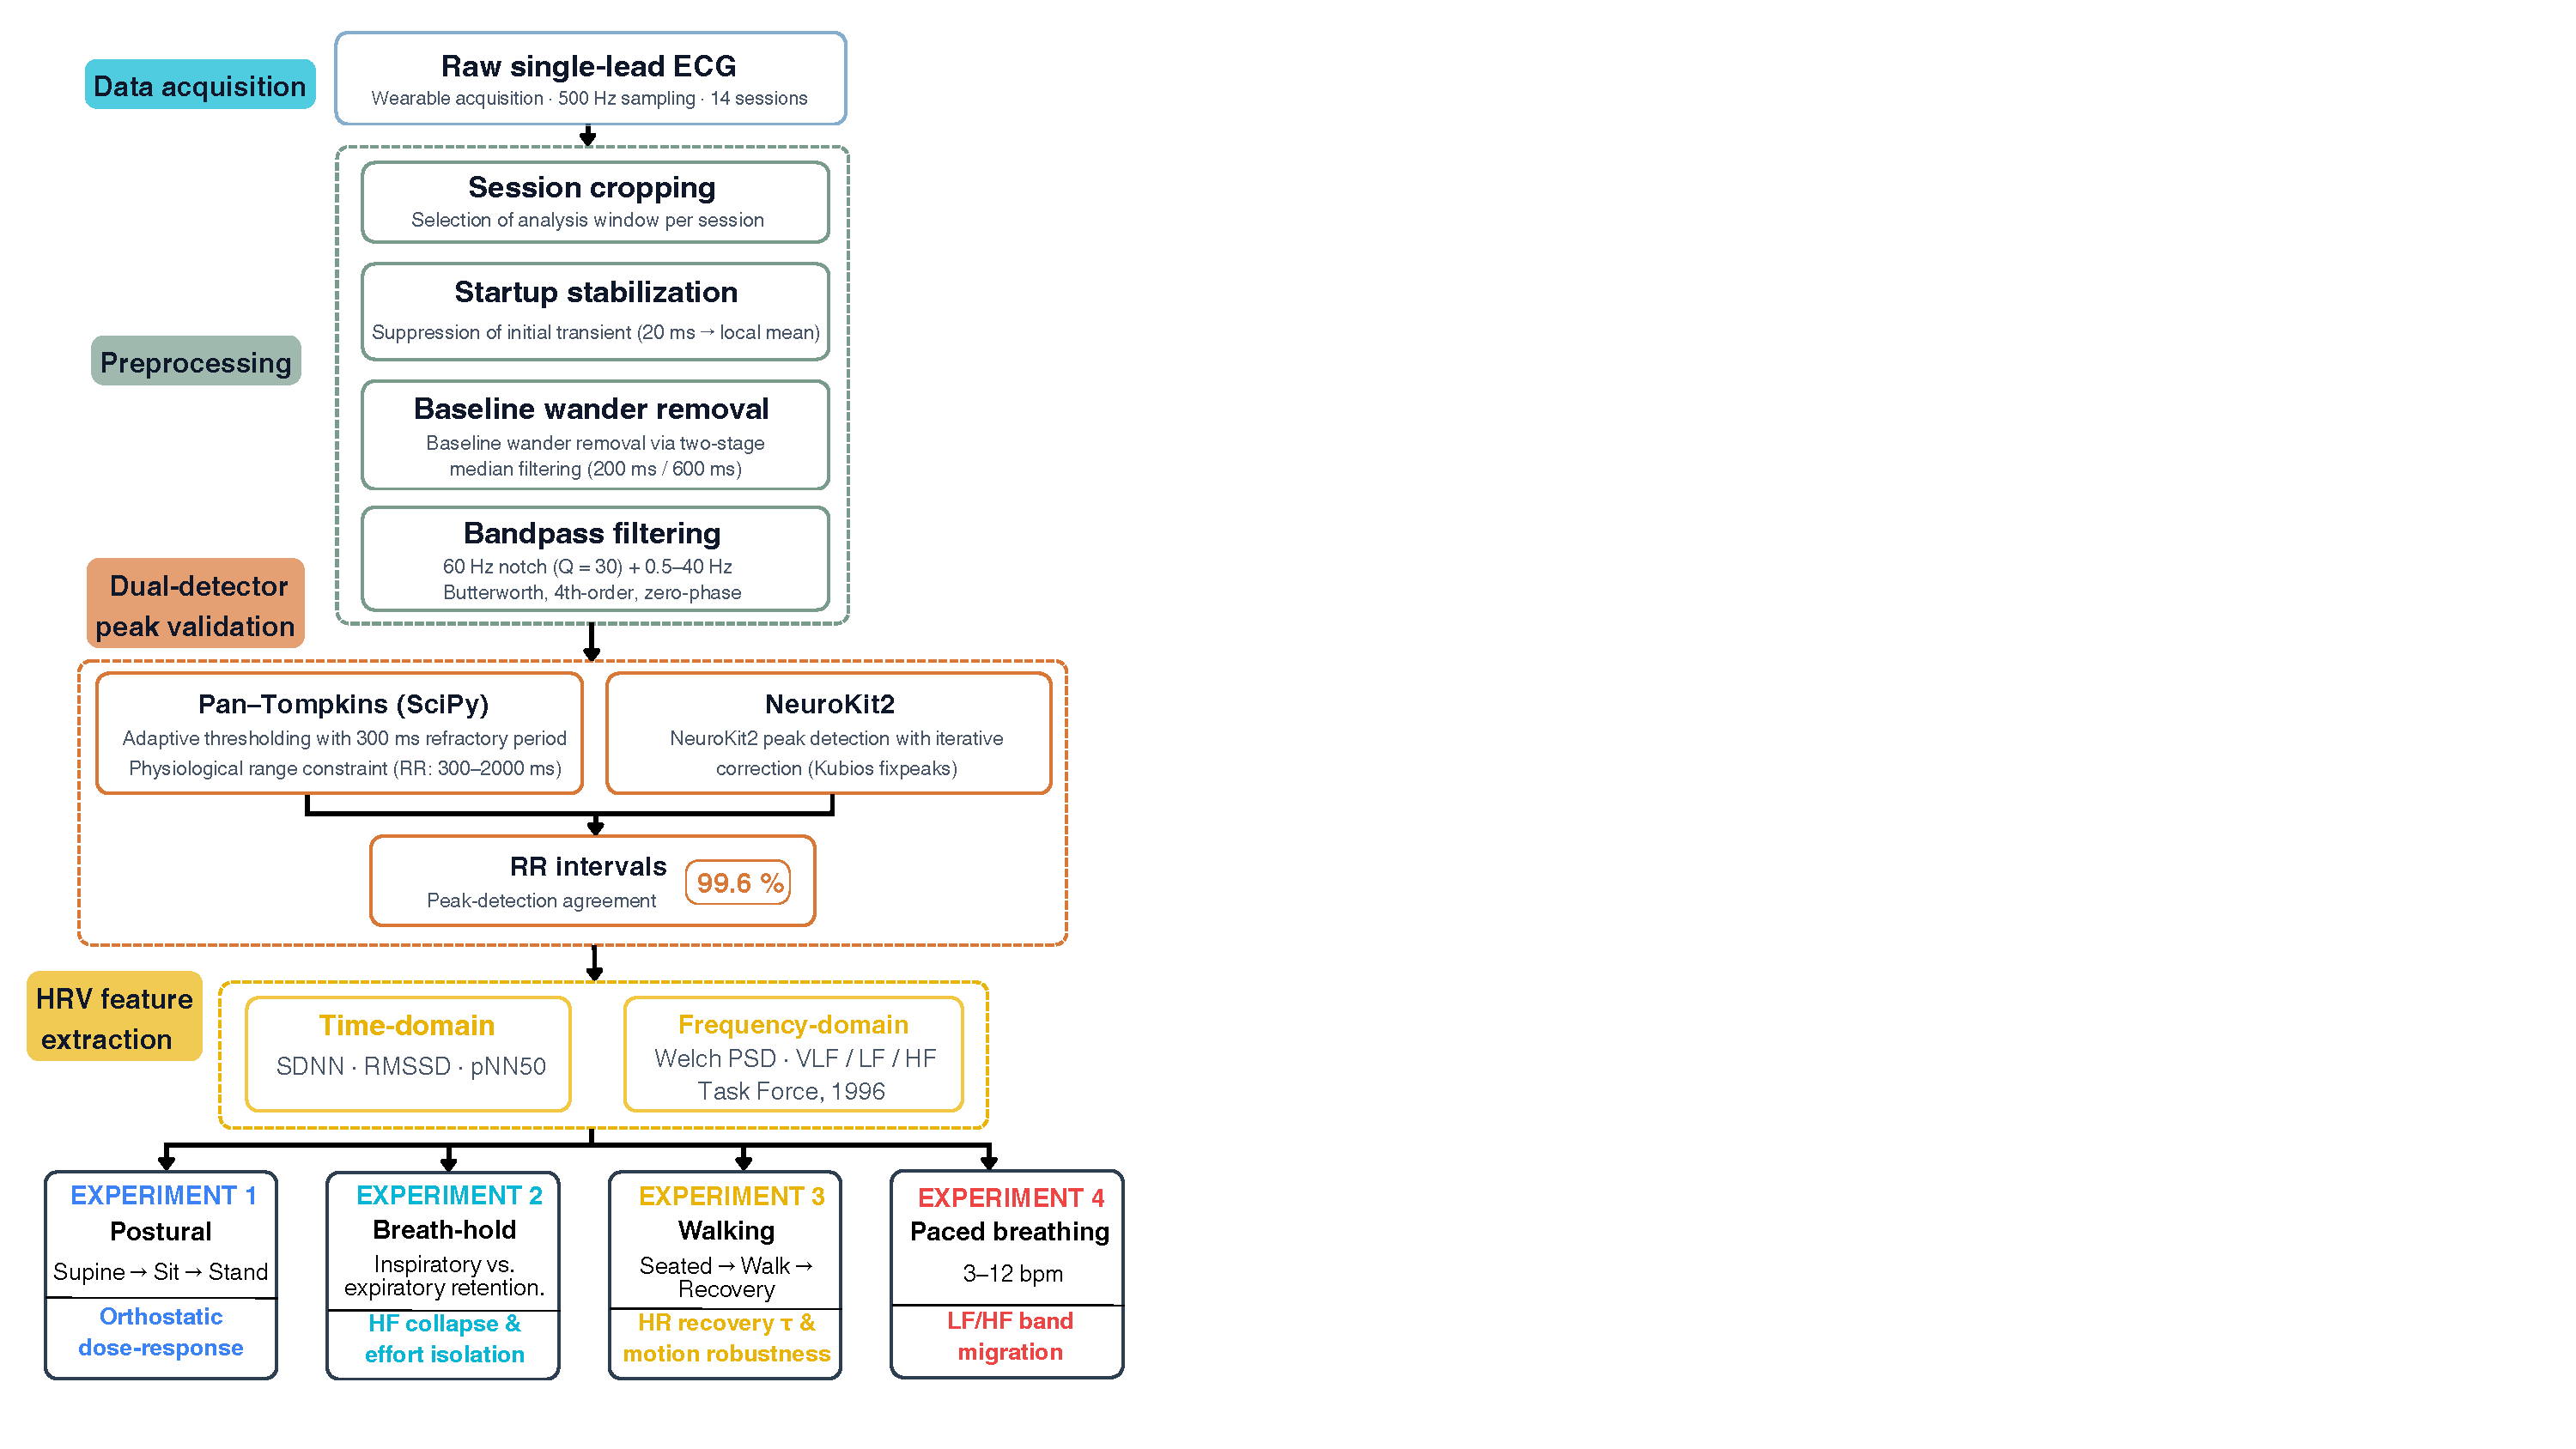
\includegraphics[width=0.64\textwidth]{nb01_fig01_pipeline_overview.pdf}
\caption{Analysis pipeline for 14~single-lead ECG recordings (500~Hz, one
participant). After cropping, baseline correction, and bandpass filtering,
R-peaks are detected in parallel by NeuroKit2 (primary) and a
Pan-Tompkins-style SciPy validator (99.6\% peak-count agreement, supine
baseline). RR-derived time- and frequency-domain HRV features feed four
experiments: postural transitions, breath-hold, walking with recovery, and
paced breathing (3 to 12~breaths/min).}
\label{fig:pipeline}
\end{figure}

% ============================================================
\section{Background: The LF/HF Ratio and Its Critique}

Malliani et~al.~\cite{malliani1991} framed LF/HF as an index of
sympathovagal balance, using LF (0.04--0.15~Hz) and HF (0.15--0.40~Hz)
bands later formalized by the Task Force~\cite{taskforce1996}. In this
study, \textbf{LF/HF} denotes the ratio of LF to HF RR power;
\textbf{RMSSD} denotes the root mean square of successive RR differences;
and \textbf{coherence} ($C_{xy}$) quantifies IMU--HR coupling at the
imposed breathing frequency.

Eckberg~\cite{eckberg1997} challenged the reciprocal framework, arguing
that LF power receives substantial vagal contribution.
Billman~\cite{billman2013} summarized two central limitations: first,
respiration can alter both LF and HF power, making LF/HF sensitive to
respiratory-band migration; second, LF power is not a selective marker of
sympathetic activity, since baroreflex-mediated vagal modulation also
contributes to the LF band. Bernardi et~al.~\cite{bernardi2000} showed that changes in breathing can
shift respiratory power into LF and distort LF/HF interpretation when
respiration is not recorded. Laborde et~al.~\cite{laborde2017} subsequently translated
these critiques into practical reporting recommendations for short-term
HRV.

Fig.~\ref{fig:hook} summarizes the study dataset. Postural loading
shifted the autonomic operating point toward higher HR and lower RMSSD.
Paced breathing, in contrast, expanded oscillatory power at nearly
constant HR and produced an 80-fold LF/HF range (0.22--17.46).

\begin{figure}[!t]
\centering
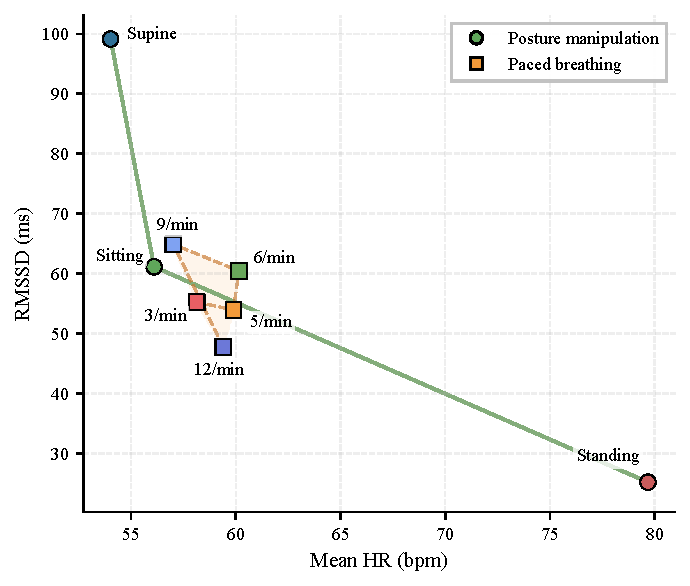
\includegraphics[width=0.48\textwidth]{fp_autonomic_scatter_hr_rmssd.pdf}
\caption{Cross-experiment operating map in the RMSSD--mean-HR plane. Green
circles, postural conditions (supine, sitting, standing); orange squares,
paced-breathing conditions (12, 9, 6, 5, 3~breaths/min). Posture moves the
operating point along a HR--RMSSD trade-off (rising HR, falling RMSSD from
supine to standing), whereas paced breathing varies RMSSD at nearly constant
HR ($\approx$57--60~bpm). The LF/HF range observed over these conditions
(0.22--17.46; Sections~3 and~5) is thus produced by task manipulation alone
and is not plotted on these axes.}
\label{fig:hook}
\end{figure}

% ============================================================
\section{Rechecking Billman's Criteria}

We focus on the two most consequential of Billman's critiques and test
each against the paced-breathing and postural data.

\subsection{Criterion 1: Respiration Alters Both LF and HF}

Billman~\cite{billman2013} argued that when respiratory frequency falls
below 0.15~Hz, the dominant respiratory oscillation migrates from HF into
LF, inflating LF/HF without autonomic change. Our paced-breathing
experiment (12, 9, 6, 5, and 3~breaths/min) provided a clear
within-subject example of this pattern.

As breathing slowed from 12/min (0.20~Hz) to 3/min (0.05~Hz), the
dominant RR spectral component closely tracked the imposed rate
($R^2 = 0.998$, residual SD = 0.003~Hz) and moved toward or across the
fixed 0.15-Hz LF/HF boundary. LF/HF rose from 0.22 to 17.46, an
80-fold increase within the same seated posture, while RMSSD remained
between 47.7 and 64.9~ms throughout (Fig.~\ref{fig:lfhf}b). Stable
RMSSD does not prove unchanged vagal tone, but it gives no evidence of
large cardiac vagal withdrawal. Because RMSSD emphasizes short-term
beat-to-beat differences, it did not scale with the large slow-breathing
oscillation in total power, making the contrast with the 80-fold LF/HF
swing conservative. The LF/HF increase is best explained by spectral-band
assignment.

We treated the 9/min condition as a boundary case without automatic
assignment to LF or HF; the reassignment rule is described in
Section~\ref{sec:fusion}.

\begin{figure}[!t]
\centering
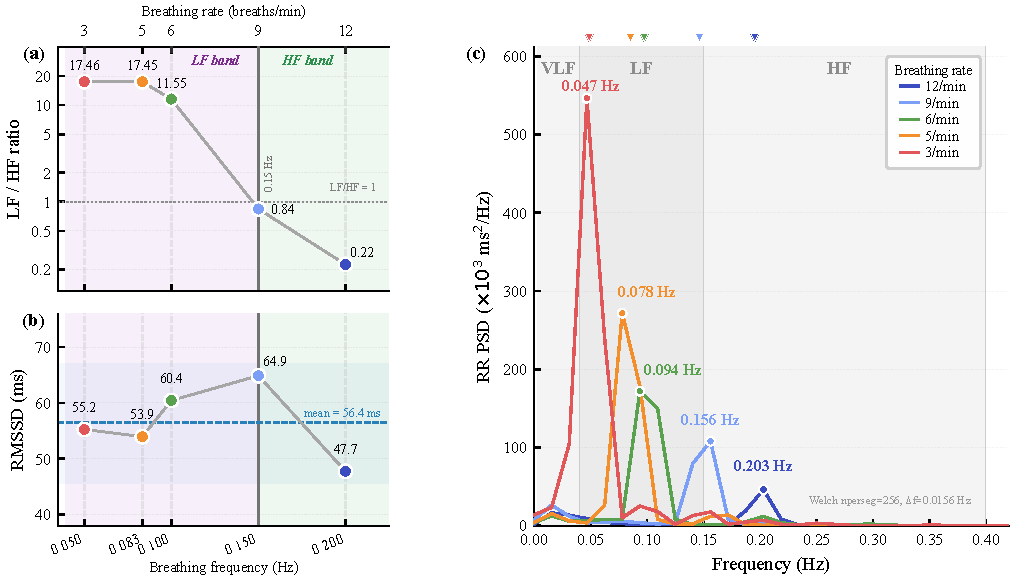
\includegraphics[width=\linewidth]{fp_lfhf_imu_summary.pdf}
\caption{Paced-breathing spectral-band migration. \textbf{(a)} LF/HF ratio
(log scale) versus breathing rate; shading marks the LF and HF bands split
at 0.15~Hz and the dotted line marks LF/HF = 1. LF/HF rose from 0.22 to
17.46 as the respiratory peak crossed from HF into LF. \textbf{(b)} RMSSD
versus breathing frequency for the same conditions, staying within
47.7--64.9~ms (mean 56.4~ms, dashed line). \textbf{(c)} RR-interval PSD for
all five rates (colour legend), computed with the canonical fusion setting
(RR interpolation $f_s = 4$~Hz, $n_{\mathrm{perseg}} = 256$,
$\Delta f = 0.0156$~Hz); VLF/LF/HF bands are shaded and top triangles mark
IMU-derived respiratory frequencies. At 9/min the metronome target was
0.150~Hz and the IMU peak 0.146~Hz, but the RR-PSD argmax used for band
assignment fell at 0.15625~Hz (HF side), so no LF reassignment was applied.}
\label{fig:lfhf}
\end{figure}

We used the synchronous triaxial IMU to test whether this band migration
reflected respiratory motion instead of an ECG-internal artifact (25~Hz
chest-patch accelerometer; Nyquist 12.5~Hz, ample for the
$\leq$0.20~Hz respiratory band). The IMU z-axis PSD peak matched the
imposed metronome frequency at all five rates, and each RR spectral peak
aligned with the IMU-measured frequency (Fig.~\ref{fig:lfhf}c).
This agreement makes a QRS-detection or preprocessing artifact an unlikely
explanation for the observed migration.

\subsection{Criterion 2: LF/HF Magnitude Alone Does Not Define
Sympathovagal State}
\label{sec:crit2}

We first establish a \textbf{positive control}. The postural experiment
(supine $\to$ sitting $\to$ standing) produced the classical orthostatic
response: HR rose from 54.0 to 79.7~bpm, RMSSD fell from 99.1 to
25.2~ms, HF power decreased from 3257 to 311~ms$^{2}$, and LF/HF
increased from 0.28 to 1.44, with the spontaneous respiratory peak
measured in each posture (0.22, 0.28, and 0.30~Hz for supine, sitting,
and standing) remaining inside the HF band
throughout~\cite{taskforce1996}. Because the respiratory peak remained in
the HF band, LF/HF changed in the expected direction for an orthostatic
challenge. This supports, but does not by itself prove, the usual
interpretation of LF/HF when the respiratory-band assumption holds.

The paced-breathing data illustrate the limitation of interpreting LF/HF
magnitude in isolation. The same participant exhibited LF/HF = 17.46
during \emph{relaxed} seated slow breathing (RMSSD = 55~ms) versus
LF/HF = 1.44 during standing (the orthostatic challenge, RMSSD = 25~ms).
The higher ratio thus appeared in the calmer condition, not in the
orthostatic challenge with its more plausible sympathetic contribution;
without respiratory context, this ordering would give an incorrect
physiological impression.

These data directly support Billman's first critique, that respiration
can move power across fixed LF/HF bands. They do not isolate the
baroreflex contribution to LF power: resolving Billman's second criterion
would require an independent sympathetic measure, such as blood pressure
for baroreflex sensitivity or pre-ejection period estimation, which lay
beyond the present single-lead ECG and IMU setup. The fusion analysis in
Section~5 provides only a partial extension by separating IMU-confirmed
respiratory power from the LF residual.

% ============================================================
\section{Rechecking Laborde's Recommendations}

Laborde et~al.~\cite{laborde2017} recommend posture-matched comparisons,
reporting of multiple HRV metrics, and explicit documentation of breathing
conditions. The present protocol follows these principles in three ways:
seated tasks are compared against a seated baseline, RMSSD, SDNN, HF, and
LF/HF are reported in parallel, and paced-breathing rates are verified
spectrally.

This reporting structure was essential for identifying the LF/HF
interpretive failure. If LF/HF had been reported alone, the 80-fold range
could be mistaken for large autonomic modulation. The parallel RMSSD and
respiratory analyses indicate that fixed-band assignment was the dominant
source of the observed LF/HF swing.

% ============================================================
\section{Multi-Sensor Respiratory Validation}

RR spectra can identify respiratory-band migration, but an independent
respiratory reference is needed to verify its origin. We therefore used the
synchronous chest-patch IMU as a mechanical respiratory surrogate.
Table~\ref{tab:fusion} summarizes IMU--ECG coupling across the
paced-breathing rates.

\begin{table}[H]
\centering
\caption{Multi-Sensor IMU--ECG Coupling Across Paced-Breathing Rates}
\label{tab:fusion}
\small\singlespacing
\setlength{\tabcolsep}{6pt}
\begin{tabular}{@{}lcccccc@{}}
\toprule
Rate & Target & IMU peak & $|\Delta f|$ & Peak $r$ & $C_{xy}$ & Phase \\
     & (Hz)   & (Hz)     & (Hz)         &          &          & ($^{\circ}$) \\
\midrule
12/min & 0.200 & 0.195 & 0.005 & 0.37$^\ast$ & 0.22$^\ast$ & --- \\
9/min  & 0.150 & 0.146 & 0.004 & 0.86 & 0.85 & +84 \\
6/min  & 0.100 & 0.098 & 0.002 & 0.76 & 0.69 & +59 \\
5/min  & 0.083 & 0.085 & 0.002 & 0.94 & 0.89 & +30 \\
3/min  & 0.050 & 0.049 & 0.001 & 0.89 & 0.83 & $-$6 \\
\bottomrule
\multicolumn{7}{@{}p{0.85\textwidth}@{}}{\footnotesize
Peak~$r$: cross-correlation at optimal lag. $C_{xy}$: magnitude-squared
coherence at imposed breathing frequency. Phase: IMU--HR lag expressed as
fraction of one breathing cycle. $^\ast$SNR-limited: fast shallow
breathing yields a weak IMU respiratory signal.}
\end{tabular}
\end{table}

\textbf{Frequency validation.} The IMU z-axis spectral peak matched the
metronome target at all five rates (mean $|\Delta f|$ = 0.003~Hz),
confirming that the chest-wall accelerometer reliably detects respiratory
motion from 3 to 12~breaths/min.

\textbf{Coupling strength.} Excluding the SNR-limited 12/min condition,
the remaining four rates (9, 6, 5, and 3~breaths/min) showed
cross-correlation $r$ = 0.76--0.94 and coherence $C_{xy}$ = 0.69--0.89,
indicating strong linear coupling between chest-wall respiratory motion
and the HR respiratory component. The 12/min condition showed weaker coupling ($r = 0.37$, $C_{xy} = 0.22$),
likely because fast, shallow breathing produced limited chest displacement
and made the IMU signal more susceptible to postural sway. This defines an applicability boundary: IMU-based respiratory validation
is most effective in the slow-breathing range where LF/HF interpretation
becomes problematic.

\textbf{Phase-frequency relationship.} Because phase equals
$360^{\circ}\times\text{lag}/T$, a roughly fixed reflex lag must produce a
phase that falls as the breathing period $T$ lengthens. This is what the data
show: phase decreased monotonically across rates, +84$^{\circ}$ (9/min)
$\to$ +59$^{\circ}$ (6/min) $\to$ +30$^{\circ}$ (5/min) $\to$
$-$6$^{\circ}$ (3/min), and the implied lag stayed near a fixed value in the
mid-range (1.0--1.6~s; mean 1.40~s over the 9, 6, and 5~breaths/min
conditions), within the 1--3~s range of cardiopulmonary/RSA reflex
latencies~\cite{hirsch1981}. The monotonic phase trend is consistent with
a fixed-lag respiratory--cardiac response and supports the physiological
plausibility of the IMU--HR coupling. It remains a secondary observation:
the 12/min condition was SNR-limited and the 3/min phase approached zero,
so per-rate phase values should not be read as precise latencies.

\subsection{Fusion-Based Recovery of the Vagal Component}
\label{sec:fusion}

The IMU validation identifies the respiratory component, but fixed LF/HF
bands still assign that component solely by frequency. We therefore used
the IMU respiratory estimate to guide a respiration-aware reassignment of
RR spectral power.

For each rate, we estimated the respiratory frequency $f_{\mathrm{resp}}$
from the IMU z-axis PSD, near the RR respiratory component. We did not use
the metronome rate for reassignment. We then integrated RR power within
$\pm \delta$ of $f_{\mathrm{resp}}$, with $\delta = 0.015$~Hz. This
window served analysis only. It corresponds to approximately one
Welch bin in the canonical fusion PSD ($f_s = 4$~Hz,
$n_{\mathrm{perseg}} = 256$, $\Delta f = 0.015625$~Hz) and should not be
interpreted as a physiological bandwidth.

For boundary cases, the reassignment decision used the RR-PSD maximum
within the IMU-anchored window. When that maximum fell in LF, the
corresponding respiratory power was classified as migrated RSA and
reassigned to the vagal pool. When it fell in HF, the original LF/HF
assignment was retained. The final band call is made by the RR-PSD argmax
rather than by the IMU peak directly because the quantity being reassigned
is RR power: the IMU only anchors the search window, so the RR spectrum
itself must adjudicate which band that power occupies.

The corrected ratio was defined as
\[
\mathrm{LF/HF}_{\mathrm{corr}} = \frac{\mathrm{LF}_{\mathrm{res}}}{\mathrm{HF} + \mathrm{RSA}_{\mathrm{LF}}},
\]
where $\mathrm{RSA}_{\mathrm{LF}}$ denotes respiratory power assigned to LF
by the fixed-band definition. For the 9/min boundary case,
$\mathrm{RSA}_{\mathrm{LF}} = 0$ under the RR-PSD argmax rule, so the
corrected ratio equals the naive LF/HF ratio.

\begin{table}[!b]
\centering
\caption{IMU-Anchored Fusion Recovery of the Vagal Component
($\delta = 0.015$~Hz)}
\label{tab:recovery}
\small\singlespacing
\setlength{\tabcolsep}{4pt}
\begin{tabular}{@{}lcccccccc@{}}
\toprule
Rate & $f_{\mathrm{resp}}$ & LF$_{\mathrm{tot}}$ & HF$_{\mathrm{tot}}$ &
LF/HF & RSA$_{\mathrm{LF}}$ & \%RSA & LF$_{\mathrm{res}}$ & LF/HF \\
     & (IMU, Hz) & (ms$^2$) & (ms$^2$) & naive & (ms$^2$) & in LF &
(ms$^2$) & corr. \\
\midrule
12/min$^\dagger$ & 0.195 & 279  & 1242 & 0.22  & 0    & 0\%    & 279  & 0.22 \\
9/min$^\dagger$  & 0.146 & 953  & 1130 & 0.84  & 0    & 0\%    & 953  & 0.84 \\
6/min  & 0.098 & 5469 & 474  & 11.55 & 2515 & 46.0\% & 2955 & 0.99 \\
5/min  & 0.085 & 7634 & 437  & 17.45 & 3516 & 46.1\% & 4119 & 1.04 \\
3/min  & 0.049 & 8980 & 514  & 17.46 & 6146 & 68.4\% & 2834 & 0.43 \\
\bottomrule
\multicolumn{9}{@{}p{0.95\textwidth}@{}}{\footnotesize
$f_{\mathrm{resp}}$: IMU z-axis respiratory peak. RSA$_{\mathrm{LF}}$:
respiratory power within $\pm\delta$ of $f_{\mathrm{resp}}$ that falls
inside LF and is reassigned to the vagal pool. For 9/min, the metronome
target was 0.150~Hz and the IMU peak was 0.146~Hz, but the canonical
RR-PSD argmax was 0.15625~Hz, inside HF. No LF reassignment was therefore
applied. The same rule applies to 12/min, where the respiratory component
also remained in HF.}
\end{tabular}
\end{table}

\begin{figure}[!t]
\centering
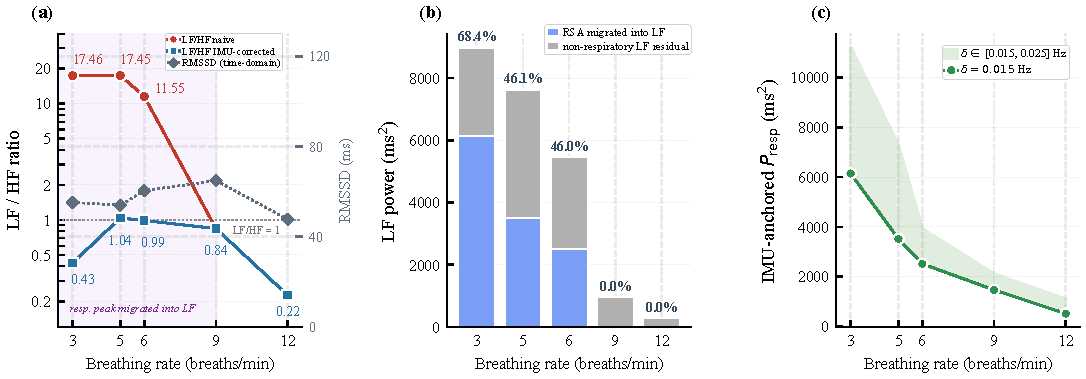
\includegraphics[width=\linewidth]{fp_fusion_recovery.pdf}
\caption{IMU-anchored fusion recovery of the vagal component. \textbf{(a)}
Naive LF/HF (an $\approx$80-fold rise across rates), IMU-corrected LF/HF,
and RMSSD (right axis, time-domain) versus breathing rate; reassignment
compressed the corrected ratio into a narrow range (0.22--1.04,
$\leq 1.05$), removing the spurious LF inflation, while RMSSD stayed
stable. The annotation marks rates at which the respiratory peak had
migrated into LF. \textbf{(b)} LF-band power split into IMU-confirmed
migrated RSA (reassigned to the vagal pool) and the non-respiratory LF
residual; the migrated-RSA share was 46--68\% at 3--6~breaths/min and 0\%
at 9 and 12~breaths/min, where the respiratory peak remained in HF.
\textbf{(c)} IMU-anchored respiratory RR power ($P_\mathrm{resp}$) versus
breathing rate, increasing as breathing slowed; the line uses
$\delta = 0.015$~Hz and the shaded band spans
$\delta \in [0.015, 0.025]$~Hz.}
\label{fig:fusion}
\end{figure}

The same pattern appeared across the slow-breathing conditions. During
slow paced breathing, IMU-confirmed RSA accounted for 46\% (6 and 5/min)
to 68\% (3/min) of LF-band power. This indicates that much of the LF
inflation reflected respiratory RSA, with no clear evidence that it
represented sympathetic modulation. Reassignment reduced the naive
$\sim$80-fold LF/HF swing (0.22--17.46) to a corrected ratio between
0.22 and 1.04 across rates, remaining $\leq 1.05$ for every
$\delta \in [0.015, 0.025]$~Hz.

After removal of IMU-confirmed RSA, the remaining LF residual gives a
cleaner estimate of non-respiratory LF power, though it is not a pure
sympathetic index. The method is a proof of concept for respiration-aware
attribution of migrated RSA power, not an estimate of absolute sympathetic
or parasympathetic tone.

\subsection{Activity-Channel Gating of HRV Validity}
\label{sec:gating}

The same IMU that recovers migrated RSA in Section~\ref{sec:fusion} flags
motion-corrupted HRV via its activity channel; we illustrate this with the
walking challenge (60~s seated, 60~s self-paced walking, 60~s seated recovery),
the only ambulatory instance in this dataset.

During walking, accelerometer RMS rose from 0.036~g (seated) to 0.103~g,
returning to 0.042~g in recovery (Fig.~\ref{fig:gating}a). The step frequency
was 1.46~Hz (88~steps/min), within 6\% of the walking cardiac fundamental
($f_0 = 1.38$~Hz); the two bands overlap in the 1--3~Hz range and cannot be
separated by linear filtering (Fig.~\ref{fig:gating}b). ECG--accelerometer
coherence at the step peak was low ($C_{xy} = 0.04$; 1--3~Hz mean $0.06$), and
the $|\Delta\text{RR}|$--motion correlation was weak ($r = 0.26$).

\begin{figure}[H]
\centering
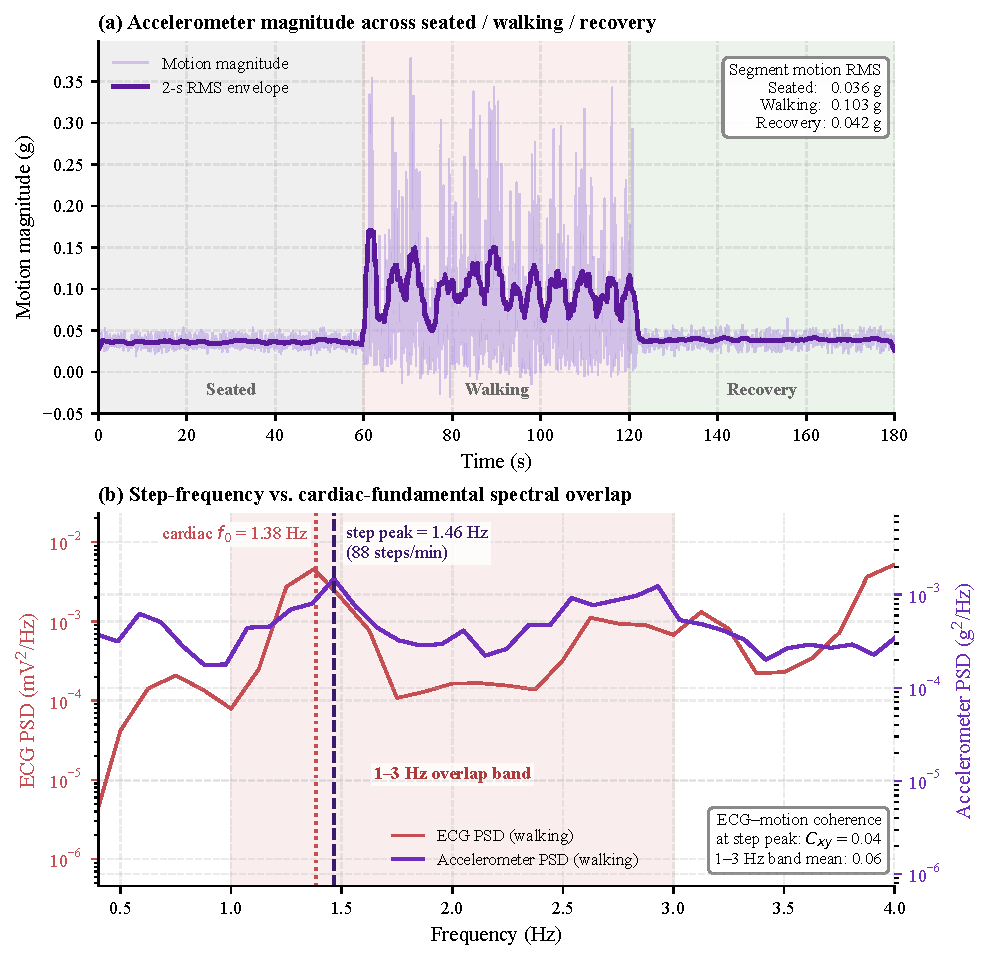
\includegraphics[width=0.72\linewidth]{fp_activity_gating.pdf}
\caption{Activity-channel gating during the walking challenge
(seated$\rightarrow$walk$\rightarrow$recovery). \textbf{(a)} Accelerometer
magnitude with its 2-s RMS envelope; segment RMS rose from 0.036~g (seated)
to 0.103~g (walking, $\approx$2.9$\times$) and fell to 0.042~g (recovery).
\textbf{(b)} Walking ECG PSD (left axis) and accelerometer PSD (right axis)
on a shared frequency axis; the step peak (1.46~Hz, 88~steps/min) lies
within 6\% of the cardiac fundamental $f_0$ (1.38~Hz), inside the shaded
1--3~Hz overlap band. ECG--accelerometer coherence is low ($C_{xy} = 0.04$
at the step peak, 0.06 over 1--3~Hz), indicating no narrowband artifact
locked into the cardiac rhythm; with the band overlap, this leaves
walking-phase fine-scale HRV motion-limited.}
\label{fig:gating}
\end{figure}

Low coherence indicates no narrowband motion artifact locked into the cardiac
rhythm, so no component can be isolated and reassigned as in
Section~\ref{sec:fusion}. It does \emph{not}, however, exclude broadband motion
drift, which the band overlap makes unremovable by filtering. We therefore treat
walking-phase fine-scale HRV (RMSSD, HF) as \emph{motion-limited} and exclude it
from cross-condition comparison; walking RMSSD (41.1~ms) is reported but not
used as a comparator. Measures independent of beat-to-beat structure remain
valid: mean HR rose from 60.8 to 83.0~bpm, with single-exponential recovery
($\tau = 6.8$~s, HRR$_{60} = 18.5$~bpm).

Across both channels, IMU--HR coherence determines the action rather than
serving as a quality threshold. High coherence with a clean respiratory line
identifies migrated RSA, which is reassigned to the vagal pool
(Section~\ref{sec:fusion}). Low coherence with step--cardiac band overlap
identifies non-reassignable contamination, so the affected fine-scale HRV is
flagged invalid. Both protect the parasympathetic estimate: the first
reattributes vagal power misassigned to LF, the second prevents a
motion-corrupted RMSSD or HF from being read as vagal tone.

% ============================================================
\section{Context-Aware HRV Reporting Checklist}

\begin{table}[!h]
\centering
\caption{Context-Aware HRV Reporting Checklist. The two right-hand columns
carry the two complementary IMU gating roles: respiratory sensing enables
\emph{reassignment} of migrated RSA power (Section~\ref{sec:fusion}), and
activity/motion gating enables \emph{invalidation} of motion-corrupted
fine-scale HRV (Section~\ref{sec:gating}).}
\label{tab:checklist}
\small\singlespacing
\setlength{\tabcolsep}{5pt}
\renewcommand{\arraystretch}{1.25}
\newcolumntype{L}[1]{>{\raggedright\arraybackslash}p{#1\linewidth}}
\begin{tabular}{L{0.15} L{0.21} L{0.13} L{0.165} L{0.185}}
\hline
Context & Preferred metrics & LF/HF use & Respiratory sensing & Activity / motion gating \\
\hline
Supine / sit / stand & HR, RMSSD, HF, LF/HF & Conditional & Recommended & Not needed \\
Breath-hold & HR, HF, recovery & No standalone & N/A (optional absence check) & Not needed \\
Walking & Mean HR, recovery $\tau$ & No & Optional & Required; RMSSD/\allowbreak HF invalid \\
Breathing $>0.15$ Hz & RMSSD, HF, LF/HF & Conditional & Optional / rec. & Not needed \\
Near 0.15 Hz boundary & RMSSD, RR PSD, $f_{\mathrm{resp}}$ & Caution & Required & Not needed \\
Slow breathing $<0.15$ Hz & RMSSD, TP, resp.\ power & No standalone & Required & Not needed \\
\hline
\end{tabular}
\end{table}

Table~\ref{tab:checklist} presents a proposed reporting framework derived
from the present single-subject case and the cited literature. The two
right-hand columns distinguish respiratory sensing for spectral reassignment
from activity gating for identifying conditions unsuitable for LF/HF
interpretation. Within this framework, LF/HF is most informative as an
autonomic-balance metric when the measured respiratory component lies clearly
within the HF band. Near 0.15~Hz, nominal breathing rate alone is
insufficient for classification. Under slow, boundary-adjacent, or
unmonitored breathing conditions, RMSSD interpreted with respiratory
monitoring provides a more defensible primary metric.

% ============================================================
\section{Limitations}

This study included only one participant. The reported LF/HF range,
coupling strength, and phase estimates therefore describe within-subject
behavior and should not be interpreted as normative values. The IMU measured
thoracic motion, not airflow, and IMU--HR coupling was weaker during fast,
shallow breathing. Respiratory peaks were estimated from per-condition
spectral windows, so within-condition drift was not assessed.

Near-boundary classification depends on spectral resolution and the
predefined integration rule, as the 9/min condition shows: under the
canonical fusion PSD the RR-PSD argmax fell one Welch bin above 0.15~Hz,
so the case was treated as a boundary and no LF reassignment was applied.
This decision does not affect the main conclusion, which rests on the
unambiguous 6, 5, and 3/min conditions: when the respiratory component
moved into LF, LF/HF lost standalone autonomic interpretability while
RMSSD remained stable. Future studies should predefine the boundary rule,
report spectral resolution, and test the method in a larger sample.

% ============================================================
\section{Conclusion}

This within-subject study shows that LF/HF can lose its intended autonomic
interpretation in short-term wearable ECG when the respiratory component
crosses fixed spectral-band boundaries. During slow paced breathing, LF/HF
varied over an 80-fold range (0.22--17.46) within a single seated posture,
while RMSSD remained stable. A synchronous IMU confirmed that the RR spectral
component followed respiratory motion. IMU-anchored reassignment compressed
the LF/HF swing into a narrower ratio range (0.22--1.04, $\leq 1.05$),
indicating that much of the apparent LF inflation reflected migrated RSA.

The same IMU also helped identify motion-limited HRV during walking. Step
motion overlapped the cardiac band and could not be isolated for
reassignment, so walking-phase fine-scale HRV was flagged as unsuitable for
LF/HF interpretation. Together, the paced-breathing and walking analyses
show that cross-channel sensing can support respiratory attribution in one
context and motion-based invalidation in another.

These single-subject observations suggest that LF/HF is most appropriate as
an autonomic-balance metric when the measured respiratory component lies
clearly within the HF band. Near the 0.15-Hz boundary, classification should
rely on the RR spectral peak within a respiratory-sensor-anchored window.
Under slow, boundary-adjacent, or unmonitored breathing conditions, RMSSD
interpreted with respiratory monitoring provides a more defensible primary
description of cardiac vagal modulation.

% ============================================================
\begin{thebibliography}{9}

\bibitem{taskforce1996}
Task Force of the European Society of Cardiology and the North American
Society of Pacing and Electrophysiology,
``Heart rate variability: Standards of measurement, physiological
interpretation, and clinical use,''
\emph{Circulation}, vol.~93, no.~5, pp.~1043--1065, 1996.

\bibitem{malliani1991}
A.~Malliani, M.~Pagani, F.~Lombardi, and S.~Cerutti,
``Cardiovascular neural regulation explored in the frequency domain,''
\emph{Circulation}, vol.~84, no.~2, pp.~482--492, 1991.

\bibitem{eckberg1997}
D.~L.~Eckberg,
``Sympathovagal balance: A critical appraisal,''
\emph{Circulation}, vol.~96, no.~9, pp.~3224--3232, 1997.

\bibitem{bernardi2000}
L.~Bernardi \emph{et~al.},
``Effects of controlled breathing, mental activity and mental stress with
or without verbalization on heart rate variability,''
\emph{J.\ Am.\ Coll.\ Cardiol.}, vol.~35, no.~6, pp.~1462--1469, 2000.

\bibitem{billman2013}
G.~E.~Billman,
``The LF/HF ratio does not accurately measure cardiac sympatho-vagal
balance,''
\emph{Front.\ Physiol.}, vol.~4, art.~26, 2013.

\bibitem{laborde2017}
S.~Laborde, E.~Mosley, and J.~F.~Thayer,
``Heart rate variability and cardiac vagal tone in psychophysiological
research: Recommendations for experiment planning, data analysis, and
data reporting,''
\emph{Front.\ Psychol.}, vol.~8, art.~213, 2017.

\bibitem{hirsch1981}
J.~A.~Hirsch and B.~Bishop,
``Respiratory sinus arrhythmia in humans: How breathing pattern modulates
heart rate,''
\emph{Am.\ J.\ Physiol.}, vol.~241, no.~4, pp.~H620--H629, 1981.
\end{thebibliography}

\end{document}
